%\documentclass{sigplanconf}
\documentclass[preprint]{sigplanconf}

\usepackage{amsmath}
\usepackage{graphicx}

%The recommended citation style is the author-date form: set up preamble
\usepackage{natbib}
\bibpunct();A{},
\let\cite=\citep

\begin{document}

\conferenceinfo{ICFP '07}{October 1-3, 2007, Freiburg, Germany} 
\copyrightyear{2007} 
\copyrightdata{[to be supplied]} 

\titlebanner{}      % These are ignored unless
\preprintfooter{}   % 'preprint' option specified.

\title{The Gem Cutter -- A Graphical Tool for Creating Functions in the Strongly-typed Lazy Functional Language CAL}

\authorinfo{Luke Evans\and Bo Ilic\and Edward Lam}
           {Business Objects}
           {\{luke.evans, bo.ilic, edward.lam\}@businessobjects.com}

\maketitle

\begin{abstract}
The Gem Cutter is a graphical tool for creating functions in the
Haskell-like language CAL by snapping together previously created
functions on a canvas known as the table-top. Our contribution is a
new graphical model supporting the composition of higher-order
functions, creation and use of local functions and variables,
composable editors for editing values of possibly compound type,
and incorporation of textual CAL
expressions. The resulting graphical representation is powerful enough
to express any CAL function, but at the same time uses few distinct
kinds of graphical elements that are organized as a set of trees
rather than a graph. The model is checked by the underlying functional
compiler at each stage, ensuring that only valid operations are
permitted. The Gem Cutter can suggest valid subsequent compositions to
various degrees of granularity. Any part of the model can be run, with
value entry for required arguments prompted for using the composable
type-directed value editors.
\end{abstract}

%\category{CR-number}{subcategory}{third-level}

%\terms
%term1, term2

\keywords
functional languages, visual programming languages, Haskell

\section{Introduction}
\label{sec:intro}

{\it CAL} is a general-purpose, lazy, strongly-typed functional
language targeting the Java virtual machine.  CAL's core is a pure
functional language that is syntactically similar to the language
Haskell and supports essentially all of the non-syntactic sugar
features of Haskell 98 with its standard addendums \cite{haskell98}.
However, CAL also closely integrates with Java; any Java class can be
imported into CAL as a CAL type, and any Java method, field or
constructor can be imported as a CAL function. Impurity in CAL arises
from calling impure imported Java entities from within CAL code.

The {\it Gem Cutter} is a development environment for a visual
programming language used to create and run CAL functions. CAL and the
Gem Cutter are together part of the {\it Open Quark Framework for Java}. In
addition, the Open Quark Framework includes Java APIs for interacting
with CAL, a supporting tool to run CAL expressions interactively from
a command line shell ({\it ICE}), and services for packaging CAL
programs as Java JARs, creating and managing metadata, and managing
resources (both CAL and client application specific).

The Quark Framework's Java API allows clients to programmatically
create CAL functions and other entities such as modules, type
definitions, type class definitions and class instance definitions. It
also exposes various type-checking operations such as unification and
pattern matching.  The Gem Cutter is a Java Swing application written
using the Quark Framework's Java API.

The main motivation for the Open Quark Framework was to create a
system capable of efficient dual language development in which CAL
could be used to define declarative business models and these models
could then be assembled by Java client programs responsible for UI,
communications protocols, interfacing to databases, security, legacy
applications, etc. The assembled models would then be validated
statically and then could be executed by the CAL compiler as a kind of
functional language based meta-programming. The initial motivation for
the Gem Cutter was as a proof-of-concept that in fact this was
possible, as the Gem Cutter is a rather general, but canonical, application of this
sort. Later, some of the benefits mentioned below provided additional
motivation for us.

In this paper we explain the key new ideas in the Gem Cutter for
people already familiar with Haskell or similar. We do not
describe (or describe only in passing) features of the Gem Cutter
typical of interactive development environments. In addition, we describe
certain implementation details not needed by end-users.

The Quark Framework for Java, including the Gem Cutter, was developed
by the Research Group at Business Objects with most actual development
work occurring with varying intensity between 2000 and the present (March 2007). The
framework is available with full sources, documentation and videos under a BSD
license at {\tt http://labs.businessobjects.com/cal/}
\cite{quarkLabsSite_withNoteOnVideos}. The videos are the best way to get a
sense of the dynamic and interactive nature of the Gem Cutter. 

The Gem Cutter is very effective for exploring and
testing the functionality of CAL modules and creating prototypes. It
is commonly used by approximately 10 experienced CAL developers at Business Objects
outside the Open Quark team as a functional laboratory to explore new
ideas -- with the considerable help of compiler feedback (e.g.\ type
inference) and its interactive, assistive features. Such users typically
create customizations involving snapping together up to 30 or so
functions. 

For experienced developers such as these, the Gem Cutter is 
mainly used in conjunction with editing CAL modules in a traditional
text-based IDE such as the CAL Eclipse plug-in.
Functions created by the Gem Cutter generate CAL text within a module
which the programmer then may modify or expand
upon. They can then go back to prototyping and testing within the 
Gem Cutter. Users sometimes discover, through the visual feedback given
by the Gem Cutter, that the functions or parts of functions that they
have been creating are more general than their specific application context.
This helps them discover useful abstractions in their work. 

In addition, we have seen the Gem Cutter used successfully by
approximately 15 developers learning functional programming for the
first time prior to actually learning any textual syntax. The
tight-feedback and interactive nature of the tool helps people to
visualize and quickly develop an intuition for the functional
programming paradigm.

We have also successfully used the Gem Cutter when presenting
business-oriented modules developed at Business Objects (and not part
of the Open Quark release) to technical decision-makers not versed in
functional programming, in 5 different application scenarios. We think
of these modules as domain specific languages for a particular
business domain. The simplicity of the graphical language means that the
presented model can be understood and people are amazed that it is
actually working code that can be run.

We feel that the lazy strongly-typed nature of the underlying CAL
language is one of the main reasons why the Gem Cutter
is so easy to use, and yet powerful enough for users to actually
express non-trivial compositions of functions without getting lost in
complex graphical representations. 

Our main new contributions are:
\begin{enumerate}
  \item
    {\it burning} -- a visual generalization of partial application.
  \item
    {\it collectors, emitters and argument retargeting} -- a visual
    representation of local functions not involving cyclic graphs yet
    powerful enough to represent direct recursion. The mechanism
    permits editing of local functions along with the top-level
    function in a single view.
  \item
    {\it value entry} -- an extensible type-directed composable method
    for entering compile-time and run-time values, as well as
    decomposing those values. Higher-order types and polymorphic types
    are both supported and customized editors can be introduced for
    polymorphic types as well as monomorphic types. In addition, the
    mechanism supports transforming values in response to changes in
    type.
  \item
    Considering burning when suggesting functions for
    connection and making use of a new measure of the quality of unification
    called {\it type closeness} to categorize how apt a connection will be,
    as demonstrated in {\it Intellicut}.
  \item
    The ability to integrate CAL textual expressions within the visual
    model using a minimal syntax that handles arguments implicitly and
    that is robust with respect to invalid expressions or connections, as
    manifested in {\it code gems}.
  \item
    The ability to include test code in the visual representation
    while not affecting the efficient representation of the actual
    generated function. This facility also allows saving of partially
    formed visual representations for which editing can be resumed
    later.
  \item
    A mature freely-available BSD-licensed open-sourced visual
    programming language taking special advantage of the underlying
    strongly-typed lazy functional language.
\end{enumerate}

All figures in this paper are portions of actual screenshots from the
Gem Cutter application with some edits for the sake of
presentation. Specifically we have resized some
value editors to remove whitespace, composited and slightly
repositioned tooltips, and removed user written documentation from
tooltips (other than the tooltips in Figure~\ref{fig:zipWithFigure}).

\section{The Graphical Language of the Gem Cutter}
\label{sec:gemcutter}

The Gem Cutter starts up with respect to a CAL {\it workspace}. The CAL
workspace defines a pre-existing set of CAL modules that form the
initial environment for a Gem Cutter session. Typically, the modules
in the workspace have been written by hand in CAL, but there may be
some modules, or parts of modules, that were created during previous
sessions in the Gem Cutter. The Gem Cutter also maintains a
notion of the {\it current module}, into which newly created entities will
be placed and that determines which modules are visible and useable in
a Gem Cutter design.

A {\it gem} is simply a CAL function, class method or data constructor,
together with any metadata attached to it. Gems can be snapped
together, or composed (via function composition) on the Gem Cutter
table-top to create new gems.

For example, Figure~\ref{fig:zipWithFigure} shows the representation of
the
\begin{verbatim}
List.zipWith :: (a -> b -> c) -> [a] -> [b] -> [c]
\end{verbatim}
gem on the table-top. It takes three
arguments, represented by the three circular input connectors, and has
an output with an arrow connector. Hovering the mouse over the inputs,
output or body of the gem produces tooltips with some information
about the appropriate part of the gem. The tooltip text is based on
the definition of the gem (such as type information), any {\it CALDoc}
(similar to Javadoc) and also any custom deployment metadata for the
gem. Color is used as a secondary hint on types in that connectors
with the same color have the same type (where type variables are
quantified over the connector's type, so that the {\tt list1}, {\tt list2} and
output connectors have the same color for {\tt [a]}, {\tt [b]} and {\tt [c]}).

\begin{figure}[htb]
  \centering
  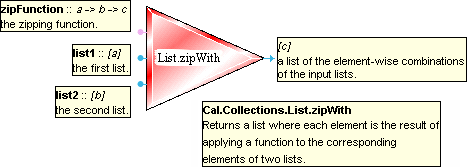
\includegraphics[width=20pc]{zipWithFigure.png}
  \caption{The {\tt List.zipWith} gem.}
  \label{fig:zipWithFigure}
\end{figure}

The {\it number of arguments} of a gem is defined as the number of top-level
function type constructors in its type. In particular, it does not
depend on the number of lexical arguments used in the gem's definition
in CAL source. For example, if the {\tt zip} function is defined as:
\begin{verbatim}
zip = List.zipWith Prelude.tuple2;
\end{verbatim}
then since its type is {\tt [a] -> [b] -> ([a, b])} it would appear
on the table-top as a two argument function even though it has zero
lexical arguments.

When there are multiple gems on the table-top, type variable names
change to indicate independence. For example, if the {\tt List.take} gem and
another {\tt List.zipWith} gem are placed on the table-top, their tooltips
will indicate types such as {\tt Int -> [d] -> [d]} and
{\tt (e -> f -> g) -> [e] -> [f] -> [g]} respectively.

Gems can be connected provided they are {\it
type compatible}. Type compatibility essentially means that the type
of the output being connected is unifiable with the type of the input
being connected to. However, there are some additional considerations
described later, related to partial applications as well as global type
constraints. If the types are not compatible then the Gem Cutter
disallows the connection.

When a valid connection is made, polymorphic types specialize as
appropriate.  For example, we can connect the
\begin{verbatim}
String.toList :: String -> [Char]
\end{verbatim}
gem to the second argument of the
\begin{verbatim}
List.filter :: (a -> Boolean) -> [a] -> [a]
\end{verbatim}
gem to produce Figure~\ref{fig:filterStringToList}.
(Note that in CAL the {\tt String} type is a foreign type with implementation
{\tt java.lang.String} and is not an alias of {\tt [Char]}).
The resulting composition defines the function:
\begin{verbatim}
f keepIfTrueFunction stringValue =
    List.filter keepIfTrueFunction
        (String.toList stringValue);
\end{verbatim}

\begin{figure}[htb]
  \centering
  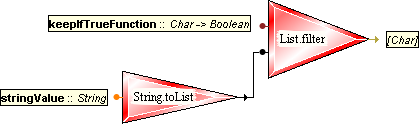
\includegraphics[width=20pc]{filterStringToList.png}
  \caption{Connecting the {\tt String.toList} gem to the {\tt List.filter} gem.}
  \label{fig:filterStringToList}
\end{figure}

Notice how the types of the {\tt List.filter} argument and the return
type have specialized to involve {\tt Char}. Note also that the
{\tt String.toList} gem cannot be connected to the first argument of
{\tt List.filter} because of type incompatibility.

An important invariant of the graphical model is that an input 
is either disconnected or has at most one connection from an output.
Similarly, an output is either disconnected or connected to at most one input.
The output of a gem cannot be connected to any input in the tree
in which the gem is located. Gems have exactly one output. The target and
collector special gems described below have zero outputs. All other special
gems described below have one output. As a result, it is only possible
to create sets of trees in the graphical model. This graphical model is
simple for users to understand and visualize. However, it is also expressive,
being able to represent sharing, recursion, local functions, etc.,
as explained later on in the paper.

The Gem Cutter automatically manages the types of all gems and
compositions on the table-top. The user does not need to assert or
declare types, an important feature derived essentially from the fact
that the underlying CAL language supports Hindley-Milner style type
inference extended with type classes, as with Haskell. Indeed, types
are used to ensure that all compositions created on the table-top are
at least structurally valid in that they correspond to CAL functions
that compile successfully.

\subsection{Burning}
\label{sec:burning}

To allow for functional return types, which are essential in composing
gems where the destination argument has a function type, we introduced
the concept of {\it burning}. Any of the arguments of a gem may be
burnt, in which case it is not available for other gems to connect
to. For example, burning the first and third argument of {\tt zipWith}
produces Figure~\ref{fig:zipWithBurnt}.

\begin{figure}[htb]
  \centering
  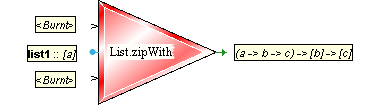
\includegraphics[width=20pc]{zipWithBurnt.png}
  \caption{The {\tt List.zipWith} gem with its first and third arguments burnt.}
  \label{fig:zipWithBurnt}
\end{figure}

The burnt arguments are displayed in a singed form to indicate that no
connection is possible to them. This graphical representation is also
interpretable as a right arrow, sending the argument to the
output. Their effect is reflected in the new functional return type of
the burnt gem: {\tt (a -> b -> c) -> [b] -> [c]}.

This graphical representation can be thought of as representing the CAL function:

\begin{verbatim}
f list1 = (\zipFunction list2 ->
    List.zipWith zipFunction list1 list2);
\end{verbatim}

Burning can be thought of as a graphical generalization of partial
application. Burning a consecutive sequence of arguments up to and
including the final argument corresponds to a partial application. For
example, burning the last argument of {\tt List.zipWith} can be
thought of as representing the function:

\begin{verbatim}
f zipFunction list1 =
    List.zipWith zipFunction list1;
\end{verbatim}

The combination of representing gems with a predictable number of
arguments while also allowing for effective use of higher-order
functions in creating new gems is of critical importance to the
ability of users to create non-trivial gems but at the same time
understand the visual representation presented to them. We view this
as one of our key contributions.

As a general observation, composing functions is simple in graphical
languages while applying functions is more awkward. The opposite is
true of textual languages, where application is simple
(e.g.\ juxtaposition in Haskell and CAL) while composition is more
awkward, typically involving lambda expressions. Burning aids in
making application more convenient in the graphical environment.

When connecting gems, if the source output and destination argument
types are not unifiable, but they would become unifiable after
burning, the Gem Cutter automatically does the burning. For example, in Figure~\ref{fig:burntConnection}, 
the argument of {\tt Char.isUpperCase :: Char -> Boolean} was
automatically burnt when connecting to {\tt List.filter}. As a visual
indicator, the mouse cursor changes to a flaming torch icon
as the user makes the connection.

\begin{figure}[htb]
  \centering
  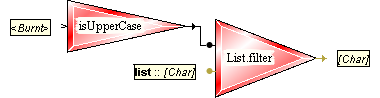
\includegraphics[width=20pc]{burntConnection.png}
  \caption{The argument of {\tt Char.isUpperCase} is automatically burnt when connecting to the {\tt List.filter} gem.}
  \label{fig:burntConnection}
\end{figure}

If there is more than one possible burning, such as when trying to
connect the {\tt Prelude.lessThan :: Ord a => a -> a -> Boolean} gem
to the first argument of {\tt List.filter}, then the connection is
prevented, but an ambiguous burn icon is displayed to indicate that
the user can choose to make it succeed by selecting the appropriate
burning.

An important point is that burning an argument is defined in terms of
the immediate gem that the argument belongs to and not the composition
as a whole. For example, burning the argument {\tt stringValue} in the
composition of {\tt String.toList} with {\tt List.filter} shown in
Figure~\ref{fig:filterStringToList} breaks the connection between {\tt
String.toList} and {\tt List.filter} (if the user proceeds after a
warning); it does not change the output type of {\tt List.filter} to
be {\tt String -> [Char]}. This is necessary so that when further
compositions are made, there are no implicit groupings of gems with
respect to which the burning is defined, but rather the meaning
of the burning is immediately clear. It is possible however to have
the effect of burning non-locally by creating a local gem (an {\it emitter}
-- Section~\ref{sec:collectorEmitter}) and burning its argument. This is described
more below.

Another way in which type compatibility is different from
straightforward unification can occur with types involving type-class
constraints. For example, in Figure~\ref{fig:globalTypeConstraints}, we
cannot connect the empty list data constructor {\tt Nil :: [a]} to the
{\tt List.sort} input even though the two types are unifiable since
there is nowhere in the resulting design to resolve the {\tt Ord}
type class constraint on the {\tt sort} input.

\begin{figure}[htb]
  \centering
  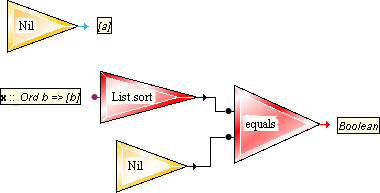
\includegraphics[width=20pc]{globalTypeConstraints.png}
  \caption{The {\tt Nil} data constructor cannot be connected to {\tt List.sort} due to a global type constraint.}
  \label{fig:globalTypeConstraints}
\end{figure}

The Gem Cutter indicates that the connection is not possible because
of a global type constraint. Fortunately, this sort of situation is
rather rare in actual practice.  On the other hand, for the {\tt Cons
:: a -> [a] -> [a]} gem (the other data constructor of the {\tt List}
type), the connection is not a problem since the {\tt Ord} type class
constraint is then reflected in the arguments of {\tt Cons} in the
resulting composition. Of course, the issues described here also occur
when writing textual expressions in CAL (or Haskell when the default
declaration for the module does not provide an ad hoc type specialization).

For many Gem Cutter operations, a local type computation is sufficient
to determine type compatibility. This means that a great many such
computations can be performed rapidly and thus the Gem Cutter can
provide assistance in suggesting what connections the user can
successfully make. Because of global type constraints, occasionally
these suggestions will be invalid, and a warning as above is given.

\subsection{Special Gems}
\label{sec:specialGems}

During the gem composition process there are certain special-purpose
entities that are used in the graphical language in creating the
resulting gem. These are the target gem, collector and emitter gems,
code gems, value gems and record field selection gems. Collectively we
call these {\it special gems}.

\subsubsection{Target Gem}
\label{sec:targetGem}

The {\it target gem} is used to define the actual gem being built on
the table-top. It can then be saved into the current module, at which
point it is available for use as a first-class gem in building up
other gems. There is always exactly one target gem on the table-top.

For example, a gem to compute the sum of squares can be defined as
in Figure~\ref{fig:sumSquares}. The lozenge-shaped special gem with
target-like markings is the {\tt sumSquares} target gem.
The gem corresponds to CAL code:
\begin{verbatim}
sumSquares list = List.sum (List.map square list);
\end{verbatim}

\begin{figure}[htb]
  \centering
  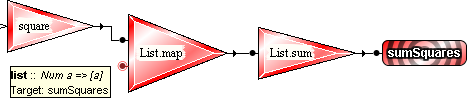
\includegraphics[width=20pc]{sumSquares.png}
  \caption{A gem design for the {\tt sumSquares} gem.}
  \label{fig:sumSquares}
\end{figure}

When a gem is saved, its defining CAL textual definition is saved in
the current module. In addition a {\it gem design} is saved. This
includes the extra metadata that are not encoded in the CAL source
definition of the function such as the positions of the gems involved
in the design.

\subsubsection{Collector Gems, Emitter Gems and Argument Targeting}
\label{sec:collectorEmitter}

{\it Collector} gems correspond to the concept of local variable or
function as defined in a let-definition in CAL source. {\it Emitter}
gems correspond to the use of that local variable or function within
an expression.

Collectors are graphically represented by black lozenge-shaped special
gems labeled with the name of the collector.

Every emitter is associated with a collector having its same
name. There can be more than one emitter associated with a single
collector. Visually, emitters are white in color, and they are
lozenge-shaped if they have zero arguments, and function-gem shaped if
they have one or more arguments.

Figure~\ref{fig:square} shows the definition of the {\tt square} gem used above
in the definition of {\tt sumSquares}. There is one collector, for
{\tt x}, and two zero-argument emitters for {\tt x}. 
This corresponds to the CAL text:
\begin{verbatim}
square x = x * x;
\end{verbatim}

\begin{figure}[htb]
  \centering
  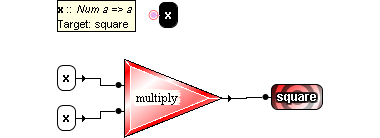
\includegraphics[width=20pc]{square.png}
  \caption{A collector gem is used in the gem design for the {\tt square} gem.}
  \label{fig:square}
\end{figure}

Once this design is saved, the {\tt square} gem can then be used like
any other gem defined via CAL source in creating further gems, as seen
in the {\tt sumSquares} design of Figure~\ref{fig:sumSquares}.

The target gem is actually a special kind of collector that corresponds to a
top-level variable or function. Emitters for the target gem are
similar to regular emitters, except they are pink to indicate that
they are top-level.

Collectors and emitters imply that the design of the gem on the
table-top may be a collection of trees, rather than just a single
tree. We call the design a {\it gem graph}. Every unbound
argument appearing on the table-top is associated with a particular
collector; we say that the argument is {\it targeted} to that
collector. In source text, this means that the argument appears as
a parameter in the definition of the function defined by the
collector. 

By default, all arguments are targeted at the target gem. An argument
may be changed to target a different collector by right clicking on
the argument to invoke a context menu and selecting a new collector to
target.

For example, in the {\tt sumSquares} design of Figure~\ref{fig:sumSquares}, the {\tt list} argument
of the {\tt map} gem is targeted to the {\tt sumSquares} target gem.

Using argument targeting, we can define {\tt sumSquares} with the
square function defined purely locally within the design, as shown in
Figure~\ref{fig:sumSquaresWithLocalSquare}.
This has corresponding CAL source text:
\begin{verbatim}
sumSquares list = 
    let
        squares x = x * x;
    in
        List.sum (List.map squares list);
\end{verbatim}

\begin{figure}[htb]
  \centering
  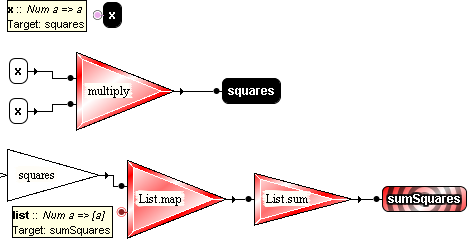
\includegraphics[width=20pc]{sumSquaresWithLocalSquare.png}
  \caption{A gem design for the {\tt sumSquares} gem with a locally defined {\tt square} function.}
  \label{fig:sumSquaresWithLocalSquare}
\end{figure}

Notice that the argument to the {\tt x} collector is targeted to the
{\tt squares} collector and so {\tt x} appears as a textual parameter on
{\tt squares} and not {\tt sumSquares}.  The {\tt squares} emitter appears
as a local function with one argument. This local function is burnt in
its connection to {\tt List.map}. The {\tt list} argument of {\tt
List.map} is the only argument targeted at the {\tt sumSquares} target gem, so the
overall gem is a function of one top-level argument.

The gem model is sufficiently powerful to represent direct recursive
functions in a reasonably simple way. For example, the {\tt
sevens} gem, shown in Figure~\ref{fig:sevens}, represents an infinite
list of {\tt 7 :: Double}.
This corresponds to the CAL source text:
\begin{verbatim}
sevens :: [Double];
sevens = 7.0 : sevens;
\end{verbatim}

\begin{figure}[htb]
  \centering
  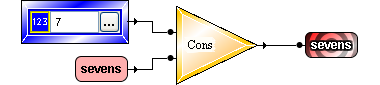
\includegraphics[width=20pc]{sevens.png}
  \caption{The {\tt sevens} gem, representing an infinite list of {\tt 7 :: Double}.}
  \label{fig:sevens}
\end{figure}

The rectangular shaped special gem with a seven in it is a {\it value
gem} (Section~\ref{sec:valueGems}), used to represent a constant value. The {\tt sevens} emitter is
connected to the list argument of {\tt Cons} in this recursive
definition.

A more elaborate example is shown in Figure~\ref{fig:demoMapDesign} in
the direct recursive definition of the gem {\tt demoMap}, which has the 
semantics of {\tt List.map}. In this design the target {\tt demoMap} gem 
is used as a two-argument emitter in its definition. The {\tt iff} gem is 
the functional form of the if-then-else expression. 
The design corresponds to CAL source text:
\begin{verbatim}
demoMap :: (a -> b) -> [a] -> [b];
demoMap mapFunction list =
    Prelude.iff (Prelude.isEmpty list)
        []
        (mapFunction (List.head list) :
         demoMap mapFunction (List.tail list));
\end{verbatim}

\begin{figure}[htb]
  \centering
  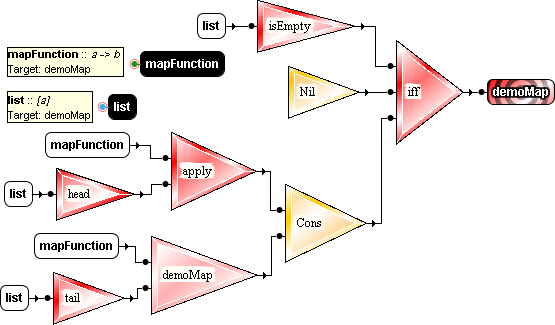
\includegraphics[width=20pc]{demoMapDesign.png}
  \caption{A gem design for the {\tt demoMap} gem, with the semantics of {\tt List.map}.}
  \label{fig:demoMapDesign}
\end{figure}

By default, target collector arguments are ordered as they would be encountered 
in a pre-order traversal of the gem graph starting at the target gem.
This would mean that the {\tt list} argument would appear before {\tt mapFunction}.
However, in this example the arguments have been reordered in the {\it arguments panel}. 
This is a separate panel that allows users to reorder the arguments of any
collector (including the target gem) so that the final gem has the
desired argument ordering.

Note that (except as explained below) the number of arguments targeted at a collector gem determines
the number of arguments of its corresponding emitter gem. This is unlike the
case of regular gems where the number of arguments depends only on the gem's type.
This is why the {\tt mapFunction} emitter in Figure~\ref{fig:demoMapDesign} appears 
with 0 arguments, even though the collector has a functional input type.
In practice, what this means is that the {\tt apply} gem occasionally is still
useful, especially in situations involving functional top-level inputs. 

As a technical side point, if an argument is targeted at a collector, and that argument's
gem tree is not used in the definition of the collector, then the argument does
not appear in the corresponding emitter. For example, adding a new collector, and
targeting its argument at the {\tt mapFunction} collector would not cause the
{\tt mapFunction} emitters to morph to having 1 argument. 

Collectors, emitters and argument targeting greatly increase the
representational power of the graphical language in the Gem
Cutter. With them, essentially any pure algebraic CAL function can be
represented given the common case that gems for decomposing algebraic
or record data type values (such as {\tt head}, {\tt tail} and {\tt
isEmpty} for the {\tt List} type) are available. The resulting
representation has the visual form of an acyclic graph with a flat
appearance permitting editing of both local functions and the top
level function in a single unpartitioned view. This contrasts with the approaches
discussed in the related works (Section~\ref{sec:related}) in which local functions
are edited in a separate window. The Gem Cutter essentially enables
this latter modality by creating a gem design, saving it, and then
reusing it in a subsequent design. However, we view this as a
secondary mechanism when snapping together small gem designs, as it is
much more convenient to have all elements of the visual design within
ready access.

\subsubsection{Collector Targeting}
\label{sec:collectorTargeting}

In addition to arguments being targeted to collectors (including the target
gem), collectors themselves can be targeted to other collectors. If a
collector is {\it targeted} to another collector, then in terms of CAL
text, this means that the definition of the first collector occurs as
a top-level let definition in the definition of the second.

Figure~\ref{fig:repeatN_collectorTargeting} shows a design that
involves non-trivial collector targeting in that the {\tt ys}
collector is targeted to the {\tt repeat} collector. The gem {\tt
repeatN} generates the following CAL text:
\begin{verbatim}
repeatN :: Int -> [a] -> [a];
repeatN nElements x = 
    let
        repeat y = 
            let
                ys = y : ys;
            in
                ys;
    in
        List.take nElements (repeat x);
\end{verbatim}

\begin{figure}[htb]
  \centering
  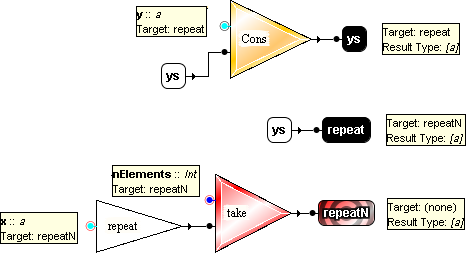
\includegraphics[width=20pc]{repeatN_collectorTargeting.png}
  \caption{A gem design that involves non-trivial collector targeting.}
  \label{fig:repeatN_collectorTargeting}
\end{figure}

An important point to note is that collector targeting affects
connectivity of gems on the table-top. For example, if another emitter
for {\tt ys} is placed on the table-top, and the {\tt repeat} emitter
is disconnected from the {\tt take} gem, then the output type of the {\tt ys}
emitter is unifiable with the type of the {\tt list} input on {\tt
take}. However, the connection would be disallowed by the Gem Cutter
because the definition of {\tt ys} is not in scope at this
level.

By default, all collectors except for the
target gem are targeted at the target gem. In practice,
targeting of collectors beyond the default is rarely needed in
the Gem Cutter. This contrasts with argument targeting which is a key
feature to allow the creation of local positive-arity functions.

\subsubsection{Code Gems}
\label{sec:codeGems}

Users can create CAL expressions and surface them as special gems
called {\it code gems}. Any arguments are automatically inferred by
the system as the user types CAL syntax.

For example, Figure~\ref{fig:quadraticFormulaCodeGem} is a code gem {\tt
quadratic} that returns the two roots of the quadratic equation
$ax^2 + bx + c = 0$.

\begin{figure}[htb]
  \centering
  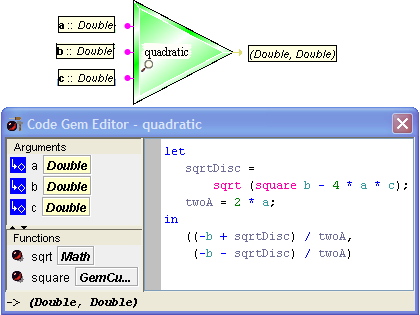
\includegraphics[width=20pc]{quadraticFormulaCodeGem.png}
  \caption{A code gem {\tt quadratic} that returns the two roots of a quadratic equation.}
  \label{fig:quadraticFormulaCodeGem}
\end{figure}

The code gem is automatically able to distinguish between the
top-level arguments {\tt a}, {\tt b} and {\tt c}, the local variables
({\tt sqrtDisc} and {\tt twoA}) and the pre-existing functions {\tt
sqrt} and {\tt square}. A pre-existing function name however can be used
instead as an argument by, for example, dragging it from the {\it Functions
list} to the {\it Arguments list}. By default, arguments appear in source
code order, but they can be reordered by drag-and-drop in the
Arguments list, as was done in this example so that the arguments are
{\tt a}, {\tt b} and {\tt c} rather than {\tt b}, {\tt a} and {\tt
c}.

Code gems can become {\it broken} by typing text that cannot
compile. In this case, the code gem takes on a cracked glass appearance.
Another way of breaking a code gem is when a previously
valid code gem that is connected to other gems is edited in such a way
that the connections become type incompatible. In this case the code
gem will break, and in addition the problem inputs or output are
highlighted. The code gem {\it locks} arguments if they are
connected, so that they remain even if the code gem text is subsequently edited to remove
the corresponding variable name. This property results in the
stability of the gem design when a code gem with
connections is being edited.
 
Code gem syntax is almost the same as the expression syntax of CAL,
with the exception that unqualified names can be used (such as {\tt
sqrt} or {\tt square}) without explicitly importing the defining
symbol. The intended interpretation of these names (e.g.\ {\tt sqrt} means
{\tt Math.sqrt} and is not an argument) is stored as additional
metadata with the code gem when the gem's design is saved.

The main new contribution in code gems is that it is possible for
users to create functions using less code than is possible within CAL
(or other similar languages) because the graphical environment makes it
easy to display and correct the assumptions made. In particular,
arguments, such as {\tt a}, {\tt b} and {\tt c} above, do not need to
be explicitly declared, and top-level functions, such as {\tt sqrt}
and {\tt square} above typically do not need to be qualified or
explicitly imported by the user. 

Another contribution is the robustness of designs involving code gems
as the code gems are edited to change or update their behavior.
This is achieved using brokenness and connection stability as described
above.

\subsubsection{Value Gems}
\label{sec:valueGems}

{\it Value gems} are used to provide a composable type-directed user
interface for creating and editing values that can be serialized as CAL textual
expressions having no free variables i.e.\ constant values. The kinds of
values that can be edited are specified in a {\it value editor registry}
file that is read when the Gem Cutter is initialized. This defines
an ordered list of {\it value editors}. A value editor essentially
specifies a list of the types for which it is able to supply values.
The ordering is used to determine which value editor to actually use
for a given type if more than one is able to handle the type.

For example, the ListTupleValueEditor handles values of type {\tt
[a]}, where the type {\tt a} can itself be edited by an embedded value
editor (the ``Tuple'' in the name is just a reminder in the code that
this editor handles lists of tuples or lists of records specially, as
a multi-column table using Swing's JTable control). 
The AlgebraicValueEditor handles values of any algebraic type.
Since CAL's {\tt List} type is an algebraic type, it
could be edited by either editor, but the ListTupleValueEditor takes
precedence because of the ordering in the value editor registry.

Currently in the Open Quark distribution, there are special
editors for CAL's string, numeric, file name, color,
relative date, relative time, relative date-time, absolute time,
enumerated (an algebraic 0-arity type all of whose data
constructors are 0-arity) and JDBC result set monomorphic types. For example, the
file name editor is simply a file chooser dialog and the date-related editors use
calendar controls. The string value editor is used for CAL's {\tt String} type as well
as {\tt [Char]} and is a text editor pane.

There are editors for record, list and range polymorphic types. Note
that tuples in CAL are a special kind of record type with field names
\#1, \#2, etc, and the record value editor is used for these. 

In addition there is the algebraic value editor mentioned above for editing
values of any algebraic type. For example, it is used for values of type
{\tt Maybe a} and {\tt Either a b}.

The mechanism is extensible, and various internal applications at
Business Objects have added their own value editors for specific
types. This involves creating a UI widget class (in Java)
implementing a specific interface, and updating the value editor
registry to include a reference to this class.

Figure~\ref{fig:valueEntry-a} shows an example of a value gem holding a
value of type {\tt [(Double, Maybe RelativeDate)]}.

\begin{figure}[htb]
  \centering
  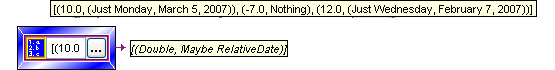
\includegraphics[width=20pc]{valueEntry-a.png}
  \caption{A value gem.}
  \label{fig:valueEntry-a}
\end{figure}

The value can be edited by clicking on the ellipsis icon. The value
editors used in creating this value are the list, record (or tuple),
numeric, algebraic (for the Maybe value), and relative date value
editors. Figure~\ref{fig:valueEntry-b} is a screenshot of editing the final
relative date value in the list, where we have opened the list, record,
algebraic and date value editors in a hierarchy.

\begin{figure}[htb]
  \centering
  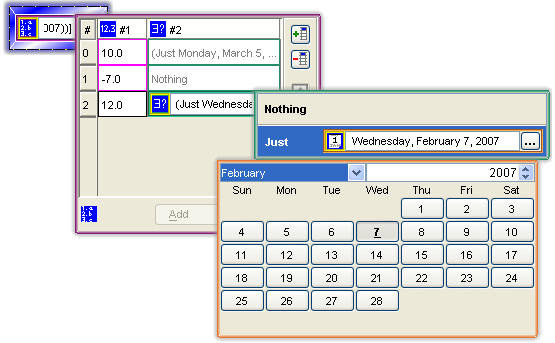
\includegraphics[width=20pc]{valueEntry-b.png}
  \caption{Composable value editors.}
  \label{fig:valueEntry-b}
\end{figure}

The value editor mechanism is also used in two other contexts within
the Gem Cutter.  Firstly, when running a gem, the value editor
mechanism is used to enter the top-level free arguments that are
needed to actually run the gem. Secondly, the output of a run gem can
be decomposed via the value editor mechanism to explore the result in
more detail.

When entering a polymorphic value, the {\it type selection editor}
lets the user choose from the types that are visible in the current
module and have value editors handling them (see
Figure~\ref{fig:typeSelection}).

\begin{figure}[htb]
  \centering
  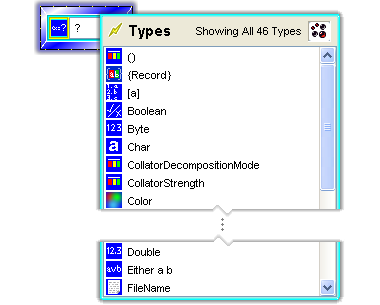
\includegraphics[width=20pc]{typeSelection.png}
  \caption{The type selection editor.}
  \label{fig:typeSelection}
\end{figure}

Type selection can be further restricted by type class constraints
as shown in the type selection editor when a value gem is connected to
the {\tt add :: Num a => a -> a -> a} gem (see
Figure~\ref{fig:constrainedTypeSelection}).

\begin{figure}[htb]
  \centering
  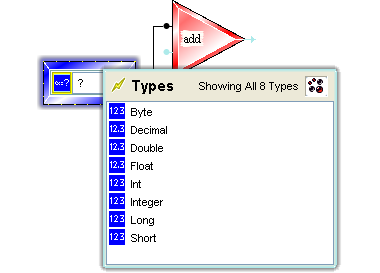
\includegraphics[width=20pc]{constrainedTypeSelection.png}
  \caption{A constrained type selection editor.}
  \label{fig:constrainedTypeSelection}
\end{figure}

Note that the value editor mechanism does not require that all values
entered be monomorphic. It is perfectly possible to enter a value such
as: {\tt (Nothing, []) :: (Maybe a, [b])}.

In most cases, if the user wants to enter values for a particular type,
it is desirable to create a custom value editor for that type. The particular support
we provide for this is a key property of our value entry system. 

One factor is simply convenience of the resulting UI. 
For example, using algebraic value editors to enter the list {\tt [True, False, True]} 
requires selecting {\tt Cons} 3 times and selecting {\tt Nil} once, in addition to 
entering the {\tt Boolean} values; this is considerably more awkward than 
using a list value editor which involves simply expanding
a list control to 3 elements and entering the {\tt Boolean} values. 
Also, the visual representation of the algebraic value editors used to enter this value
uses much more screen real-estate.

In addition, many types benefit from taking advantage of pre-existing UI
controls (such as table controls, file choosers, text edit panes, color choosers, etc.)
to provide useable value entry. These controls often suggest and facilitate the easy
entry of common values. For example, often a file name will be the name of an existing file, and
a file name chooser allows simple navigation to obtain that value. 

For algebraic types, another consideration is that typically data constructors will be private 
(to make the data type an abstract data type), and the fields of the data constructors
are subject to various design invariants ensured by constructor functions, but not possible
to ensure via direct construction using the data constructors. In this respect, types
such as {\tt Maybe}, {\tt Either} and enumerated types are atypical.

It is often useful to subset the possible values enterable to those for which
a useable UI can be given. As a simple example, when entering a value representing a conditional
formatting rule on a {\tt Double} field in a report, the underlying data type might have a field
of type {\tt Double -> Color} which will then be used to decide what color an actual value should
be displayed as in the report. We might choose to supply a UI that allows entry of values of
the form 
\begin{verbatim}
\value -> if value > constant1 then red else if
    value > constant2 then yellow else green
\end{verbatim}
i.e. it only requires the user to enter 2 {\tt Double} constant values rather than an arbitrary function.
In industry this is called a traffic light key-performance indicator. We have adopted this sort of technique
in our internal applications. Another example of subsetting is given by our use of Intellicut for run-time value
entry as described in Section~\ref{sec:valueEditorsRevisited}.

Finally, we specifically note that although value editors are composable, there are type specializations
for which we use different editors or the editors take on a special appearance. For example, values of type
{\tt [Char]} are edited with a text editor pane, and not a list value editor.
Similarly, values of type {\tt [\{r\}]} (lists of records or tuples) are edited with a table, rather than a list editor that
only shows the entire record value (as a horizontal row) for the particular list element selected.

\subsubsection{Record Field Selection Gems}
\label{sec:recordFieldSelectionGems}

The {\it record field selection} special gem is used to extract field values
from CAL records. For example, the gem shown in Figure~\ref{fig:recordFieldSelection} models the CAL expression ``{\tt
arg.\#3}'', to select the {\tt \#3} field of a record having such (such as a
triple or 4-tuple), where the user has typed the field name that they
want to select into the label on the gem.

\begin{figure}[htb]
  \centering
  
\includegraphics[width=20pc]{recordFieldSelection.png}
  \caption{A record field selection gem.}
  \label{fig:recordFieldSelection}
\end{figure}

\subsection{Running Gems}
\label{sec:runningGems}

The target gem, any collector, and indeed the gem at the root of any
tree on the table-top may be run. When this is done, the Gem Cutter
will prompt for the arguments required using {\it value entry panels}.

Figure~\ref{fig:runningGems-a} shows an example of running a gem tree
rooted in the {\tt List.filter} gem. Value editors pop up to allow the
user to enter the two arguments of type {\tt a} and {\tt [a]}
respectively. The first was specialized in the editor UI to {\tt
String} which caused the other to specialize to {\tt [String]}. The
values were then entered using the value editor mechanism described
above.

\begin{figure}[htb]
  \centering
  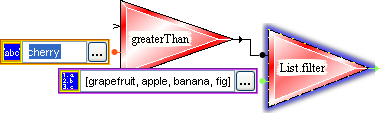
\includegraphics[width=20pc]{runningGems-a.png}
  \caption{Running a gem.}
  \label{fig:runningGems-a}
\end{figure}

Resuming the run then produces the output, which we explore in a structured
way using the value editor mechanism, as shown in
Figure~\ref{fig:runningGems-b}.

\begin{figure}[htb]
  \centering
  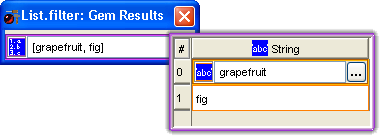
\includegraphics[width=20pc]{runningGems-b.png}
  \caption{The result of running a gem, shown in a structured way using value editors.}
  \label{fig:runningGems-b}
\end{figure}

When a collector or gem tree is re-run, any previously-entered
argument values are remembered, and used to initially populate the
UI. If the gem design is edited before being re-run in such a 
way that the argument types change, those arguments that still 
exist and have not changed type will have their previously-entered 
values remembered. Furthermore, for those arguments that have changed type, 
an attempt will be made to adapt the previous values to their new types 
(see Section~\ref{sec:valueEditorsRevisited}). 
The run mechanism also is able to abort during
execution if requested by the user.

Often there are gems on the table-top that are not used in the textual 
definition of the gem defined by the target collector. For example, these may be used in test code for
the target or for some work-in-progress. These are nevertheless saved as part
of the gem design. Figure~\ref{fig:factorialTesting} shows a test of the
{\tt factorial} gem, where running the tree rooted in {\tt List.map}
and supplying arguments $1$ and $10$ produced the list of factorials from 1 to
10. Note that the saved CAL text for this gem is simply:
\begin{verbatim}
factorial n = List.product
    (Prelude.upFromTo (1 :: Integer) n);
\end{verbatim}
and does not incorporate the test code. The ability to incorporate
tests directly within a design, while not compromising the efficiency
of the resulting code, is a contribution of this paper.

\begin{figure}[htb]
  \centering
  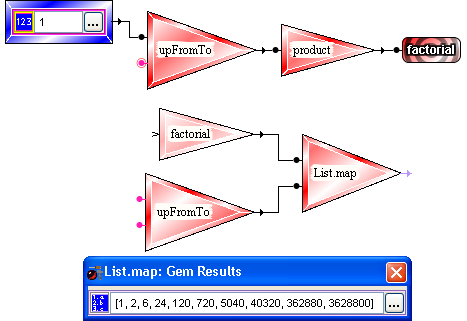
\includegraphics[width=20pc]{factorialTesting.png}
  \caption{Testing the {\tt factorial} gem.}
  \label{fig:factorialTesting}
\end{figure}

The ease with which gems, and various test fragments created from
them, can be run in the Gem Cutter is one of the biggest contributors
to the usability of the tool, especially for initial exploration and
testing.

\subsection{Intellicut and Type Closeness}
\label{sec:intellicut}

The Gem Cutter can suggest what gems can be connected to a given input
via a feature called {\it Intellicut}. The gem being connected may
need to have some of its inputs burnt to make the connection succeed,
and this is taken into account.

Figure~\ref{fig:intellicut} shows an example of applying Intellicut to the
first argument of {\tt List.filter}, which has type {\tt a -> Boolean}. We have
selected to display the ``best'' gems (see below), of which there are
55, rather than all 274 gems that would match. Note the torch icon appearing next 
to the name of each gem; this indicates that the gem connects via burning. 
The icon beside the {\tt isElem} gem is decorated with a question mark, indicating
that it requires extra user input to precisely specify the burning needed.

\begin{figure}[htb]
  \centering
  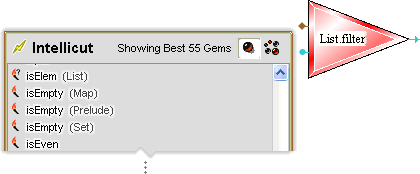
\includegraphics[width=20pc]{intellicut.png}
  \caption{An Intellicut for the first argument of {\tt List.filter}.}
  \label{fig:intellicut}
\end{figure}

To judge the suitability of a gem for connection, we introduce the concept of 
{\it type closeness}. We define a function:
\begin{equation*}
\mathsf{typeCloseness :: Type \rightarrow Type \rightarrow Int}
\end{equation*}
such that if the two argument types do not unify the return value is
$-1$. A non-negative result means that the types unify. The larger the
number, the closer the two types are in the following sense: if the
first type argument is fixed, and we consider the resulting partial
application as a function from $\mathsf{Type \rightarrow Int}$, then
the set of values attained by this function on its domain can be used
to categorize how close unification is. We use this as a heuristic to
filter the Intellicut lists into two or three different groups
(depending on the number of gems) i.e.\ the ``best'', ``likely'' and
``all compatible'' gems.

The algorithm awards one point to each step in unification when a type
constructor matches another type constructor or where a type
constructor unifies with a type class constrained type variable. For
example,
\begin{equation*}
\mathsf{typeCloseness~(\text{\tt a -> a})~(\text{\tt Int -> Int}) == 2}
\end{equation*}
There is 1 point for the match on the {\tt Function} type constructor, and 1
point for the match on the second argument of the {\tt Function} type
constructor ({\tt Int}) in the process of unification.
\begin{equation*}
\mathsf{typeCloseness~(\text{\tt Either Int Char})~(\text{\tt Eq a => a}) == 3}
\end{equation*}
There is 1 point for {\tt Either a b} conditionally being in the {\tt Eq} type class, and 1
point each for {\tt Int} and {\tt Char} satisfying the derived class constraints
{\tt (Eq a, Eq b => Eq (Either a b))}.

There are a few natural refinements to type closeness that we have not
yet pursued. The main one is to award less than 1 point for the
unification of a type constructor with a type class variable depending
on how ``exclusive'' the type class is. For example, in CAL, essentially
every type (all those whose type variables have kind *) is an instance
of the {\tt Typeable} type class. Thus unification with {\tt Typeable a => a}
is not all that special and does not deserve a type closeness
point. We plan to correct this in general by awarding fractional
type closeness points for unification with constrained type variables
depending on how many types are instances of the class.

\subsection{Value Editors Revisited}
\label{sec:valueEditorsRevisited}

The value editor mechanism can take into account that some editors are
available at run-time only (i.e.\ for value entry panels) or at
design-time only (for value gems). For example, certain values may not
have a serialized format and thus cannot be used at design-time since
the resulting gem design cannot be saved. Another example is the use
of Intellicut as a value entry panel for function values. 
At design-time, the composition of gems in the regular way offers greater 
flexibility, so this alternate mechanism is not made available.
However, at run-time this is used as a convenient way to enter higher-order
values. For example, when running the {\tt List.sortBy} gem to
sort a value of type {\tt [String]}, the value panel for the
comparator argument will suggest the {\tt Prelude.compare} and {\tt
String.compareIgnoreCase} gems using Intellicut.

Value editors also have the ability to change their types, and attempt
to convert any existing values using an extensible value
transformation mechanism. For example a value gem
holding the value {\tt [10, 20, 30] :: [Int]} can be changed to type {\tt
[String]} by invocation of a type selection editor on an element of
the list value. This will produce the value {\tt ["10", "20", "30"] ::
[String]}.

\subsection{The Scope}
\label{sec:scope}

An alternative to the representation given by the table-top is a
tree control which we call {\it the Scope}. All table-top operations,
such as connecting gems, adding special gems such as collectors and
emitters, running gems and Intellicut, can be done within this
tree-control. This is a more compact representation of the logical
structure of the table-top, and we have used this in internal
applications to embed the visual language of the Gem Cutter into
settings where less screen real estate is available.

As an example, Figure~\ref{fig:scope} shows the definition of the gem 
{\tt demoMap} in the Scope. The design for this gem was given earlier
in Figure~\ref{fig:demoMapDesign}.

\begin{figure}[htb]
  \centering
  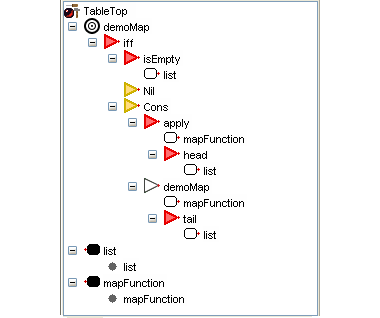
\includegraphics[width=20pc]{scope.png}
  \caption{The definition of the {\tt demoMap} gem, as shown in the Scope.}
  \label{fig:scope}
\end{figure}

\subsection{A Whole Program Business-Oriented Example}
\label{sec:wholeProgram}

\begin{figure*}[bt!]
  \centering
  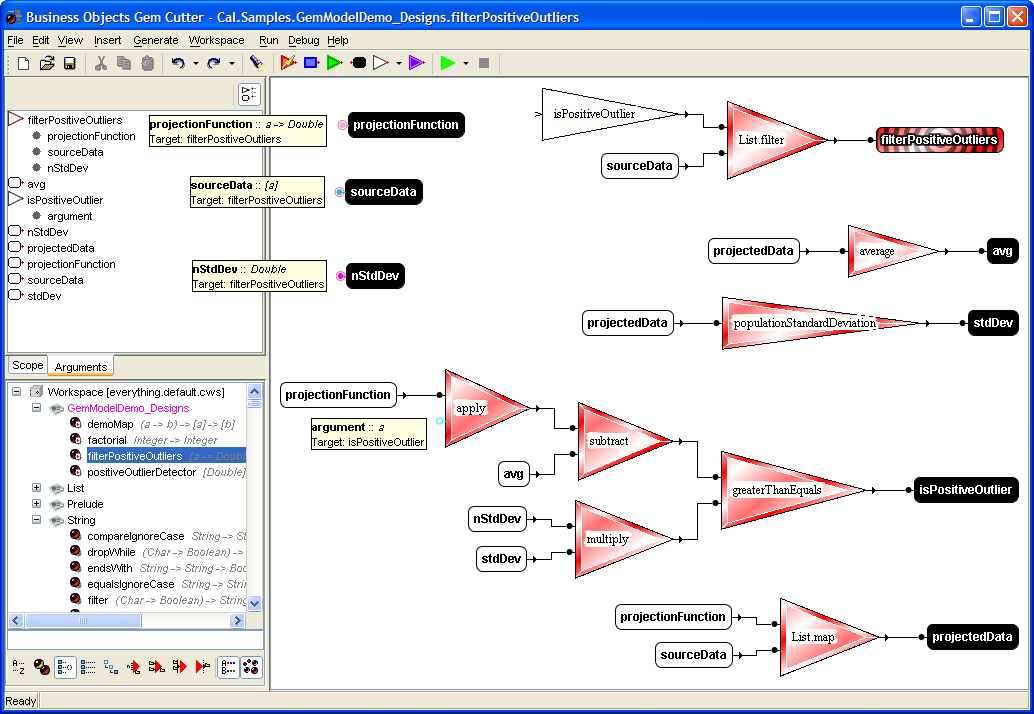
\includegraphics[width=42pc]{filterPositiveOutliers.png}
  \caption{The Gem Cutter application with the design of the {\tt filterPositiveOutliers} gem.}
  \label{fig:filterPositiveOutliers}
\end{figure*}

We now show an end-to-end example demonstrating how the various pieces
of the Gem Cutter fit together as a whole, including the arguments
panel and gem browser. We also show the use of record types in the Gem
Cutter.

Figure~\ref{fig:filterPositiveOutliers} shows the entire Gem Cutter
application with the design of the {\tt filterPositiveOutliers}
gem. This has CAL source definition:

\begin{verbatim}
filterPositiveOutliers ::
    (a -> Double) -> [a] -> Double -> [a];
filterPositiveOutliers
    projectionFunction sourceData nStdDev = 
    
    let
        avg = Summary.average projectedData;
        projectedData =
            List.map projectionFunction sourceData;
        stdDev =
            Summary.populationStandardDeviation
            projectedData;
        isPositiveOutlier argument =
            projectionFunction argument - avg
            >= nStdDev * stdDev;
    in
        List.filter isPositiveOutlier sourceData;
\end{verbatim}

This gem filters source data to return only those elements that are a
certain number of standard deviations above the mean, where a
projection function is used to provide a metric on each source data
list element. This is a more business-oriented example, and reflects
typical use of the tool internally by others at
Business Objects, as described in the introduction.

The arguments panel in the top-left of
Figure~\ref{fig:filterPositiveOutliers} shows the arguments that would
appear on any corresponding emitter for a given collector. 
The {\tt filterPositiveOutliers} target gem has 3 arguments and the
{\tt isPostiveOutlier} predicate emitter has 1 argument.
All other emitters have 0 arguments.

The bottom-left of Figure~\ref{fig:filterPositiveOutliers} shows the
{\it Gem Browser}. This shows all the pre-existing gems in the
workspace, and provides various facilities for locating
gems. Pre-existing gems can be dragged from this view onto the
table-top. Alternatively, gems may be selected by Intellicut invoked on a blank region of the
table-top (and not on an input or output), or selected via Intellicut
on an input or output as described earlier.

\begin{figure}[hbt]
  \centering
  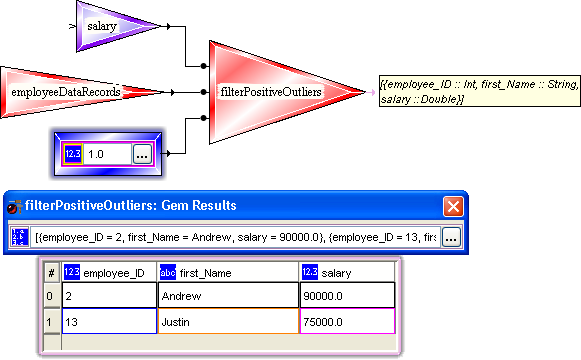
\includegraphics[width=20pc]{runFilterOutliers.png}
  \caption{Using the saved {\tt filterPositiveOutliers} gem to perform a concrete calculation.}
  \label{fig:runFilterOutliers}
\end{figure}

Figure~\ref{fig:runFilterOutliers} shows using the saved {\tt
filterPositiveOutliers} gem in a new gem graph to perform a concrete
calculation. The {\tt employeeDataRecords} gem outputs a list of CAL
records and has type {\tt [\{employee\_ID :: Int, first\_Name :: String,
salary :: Double\}]}. It was created using the Generate JDBC Data
Source wizard that composes a number of gems to access an
underlying relational data source, perform the query, and marshal to a
typed CAL list of records. Note that a record field selection gem is
used to make the filtration based on the {\tt salary} field and that a
value gem is used to input the choice of 1 standard deviation as the
filter bound. In this case the output consists of 2 records, which are
displayed using the value panel mechanism.

\section{Design Emphasis, Limitations and Future Direction}
\label{sec:designEmphasis}

The graphical language of the Gem Cutter emphasizes the creation of
functions as opposed to types, type classes or class instances. 
Pattern matching is not supported explicitly in the graphical
language; we use functions such as {\tt List.head} and {\tt
List.tail}, record field selection gems or code gems to do this.

Note that there is some support for the creation of types and type
classes in certain special cases. For example, wizards exist for
generating enumerated types deriving common type classes and
for generating CAL modules with bindings to Java classes.

The decision to emphasize functions is based on the fact that they are
overwhelmingly the most prevalent kind of entity. In the Open Quark
non-test modules there are 4249 top-level functions, 84 algebraic
types and 107 foreign types (these are Java types imported into CAL;
these must be manipulated via functions rather than pattern
matching). In particular, for the sort of prototyping and exploration
coding for which the Gem Cutter is typically used, the types have been created
already, and for the most part decomposition functions such as {\tt List.head}
are available, with a code gem workaround if not.

Nevertheless, one area of enhancement is to provide more facilities
for creating types, type classes and instances, and supporting pattern
matching more directly.

We plan a {\it record creation} special gem to model CAL expressions such as:
{\tt \{name = n, salary = s\}}. This would produce a two argument gem of type:  
{\tt a -> b -> \{name :: a, salary :: b\}}.

We also plan a {\it data constructor field selection} gem. This is similar to
the record field selection gem, but for algebraic types instead of record types.
For example, it could model the CAL expression {\tt x.Just.value}. This would
produce a gem of type {\tt Maybe a -> a} with the same behavior as {\tt Prelude.fromJust}.

A useful extension of Intellicut would be the ability to replace a
connected gem, in place, with one that is type compatible. Currently,
it is necessary to disconnect existing connections to the connected gem
to do this.

The value editor mechanism can scale poorly when used to display results
which have a large representation, such as a long list of records.
This does not typically happen for the design-time or run-time entry of
values, since data must be entered by the user. There are two different aspects
in solving this problem. One involves creating the UI controls only as needed
by the user when they explore the value. Another involves actually performing 
the underlying CAL computation lazily according to user interaction in the editor mechanism.
For example, when outputting a list of records, we may display only 30 records,
and lazily continue the computation when a user scrolls down to see more values.
The underlying CAL language has mechanisms to do this, so it is possible in principle.

The Gem Cutter supports various more standard IDE style features, such
as: the ability to add locale and application specific deployment
metadata to any CAL entity, UI wizards for generating CALDoc, CAL
source search and identifier renaming facilities, CAL source lint
detection, help facilities, and wizards for creating enumerated types,
bindings to Java classes, and bindings to JDBC data sources. We are
migrating this functionality to our CAL Eclipse plug-in, and indeed
envision the Gem Cutter's table-top itself as eventually being
available in Eclipse. In advanced usages, people alternate between editing 
Gem Cutter designs and editing of CAL source within a text editor,
refreshing the Gem Cutter to update itself with the new
contents of the workspace. We want to provide better support for this
kind of workflow.

Another area for future work is in robustness with respect to changes
in dependees. For example, if a gem design depends on a function whose
type in the meantime has changed in an incompatible way, then the
module in which the gem is defined will not compile, and the gem
cannot be loaded. Generally, if fixes are made by hand to the CAL text
of the module, the dependent gem design can be successfully loaded,
but the process is error prone. Our plan is to increase robustness
particularly in the cases where the relevant modules can be parsed but
compilation fails, such as if we delete a function required by a
particular gem design.

\section{Related Work}
\label{sec:related}

The notion of connecting up nodes in a graph to represent a function
is found in the Prograph dataflow visual programming language
\cite{cox89}. However, Prograph is an object-oriented language, and
thus the whole system is rather different from the Gem Cutter.

\citet{dami96} address the problem of higher-order function
composition (as is addressed by burning in CAL) in the different
context of an untyped visual lambda calculus. The solution is
visually significantly different from burning and involves
cyclic graph structures and structures edited within a separate view
(visually presented as substructures within a box in the paper).

VisaVis \cite{poswig94} is a higher-order visual functional programming language
visually very different from the Gem Cutter in that
composition of a higher-order function is made via substitution,
effectively dragging the body of the first function into the second.

\citet{kelso02} defines and provides an implementation of
VFPE, a dataflow visual programming language for Haskell. The website
provides some Java applets that demonstrate the system clearly and
show some of the distinctions between using it and the Gem Cutter. For
example, local definitions are defined in a separate view, arguments
are specified by typing in expressions rather than inferred from the
composition, types are displayed at outputs only for the full function
type rather than distributed across outputs and inputs. Additional Haskell
features such as explicit pattern matching are supported. Kelso's PhD thesis
also has a thorough discussion of previous related works.

Visual Haskell \cite{reekie95} is another dataflow visual
programming language for Haskell. Its visual representation is
different from that of the Gem Cutter; boxes with internal detail are
used to represent groupings of functions, there are explicitly cyclic
graph structures, and the system uses special icons for common Haskell
data constructors and functions. The dynamics of editing functions in
the system are not addressed. In addition, Visual Haskell does not
have a full implementation. However, Visual Haskell does 
support additional expression-oriented features such as pattern
matching.

The two visual dataflow languages for Haskell described above are the most
directly similar to the Gem Cutter. In general, they emphasize
completeness of the representation of the syntax of Haskell in
graphical terms. In contrast, the Gem Cutter emphasizes the actual
dynamic workflow used to create and test functions. The creation of 
local functions, use of partial application and use of higher-order
functions are particularly convenient in the Gem Cutter.

\citet{hanna02} describes the Vital system which provides the ability to edit certain
Haskell data type values visually. It has almost no intersection with
the functionality of the Gem Cutter; it is not a dataflow visual
programming language and is essentially a document management system making
explicit use of Haskell source-level definitions.

\citet{achten-afp04} have
created the GEC toolkit for constructing GUI components in a
compositional and type-directed fashion. Using the dynamic type system
support of the underlying Clean language and the Esther functional
shell, components built with the GEC enable the user to build up
complex data values through the use of type-safe composite value
editors, and to provide arbitrary higher-order expressions in source
code form, which are type-checked interactively. While this
functionality is similar to those provided by code gems and value
gems, the Gem Cutter differs from the GEC in several fundamental
aspects. The Gem Cutter is a visual development environment specifically
tailored for creating and running CAL functions rather than a general GUI building
framework. In particular, every valid gem design corresponds to a valid CAL function
definition. Also, values created by GEC-based editors must be constructed in a top-down
fashion, and cannot be composed in a more dynamic and interactive
style as provided by our graphical gem composition mechanism. 
Similarly, our value entry system is specifically tailored for entry of values
within the context of a visual programming language while the GEC is
a toolkit. Thus our mechanism supports type selection, conversion of values under
changes of type, custom value editors as the norm for editing values
in an optimal way, distinction between run-time and static values,
and the notion of providing UI for entering subsets of the legal values
of a type predicated on utility, such as provided by Intellicut.


\section{Conclusions}
\label{sec:conc}

The graphical language of the Gem Cutter provides a powerful way to
represent a wide variety of CAL functions. Our representation of a gem as having a
number of arguments dependent on its type, but allowing for partial
application via burning, is a key contribution. Our system of
collectors and emitters, and targeting of arguments to a collector,
allows even directly recursive functions to be represented in the
visual language, with a clean
representation as a simple set of trees rather than a full-fledged graph or a
view with multiple ``boxes''.  Code gems make incorporating CAL
expressions simple, without the burden of declaring variables or
function names explicitly. The advanced Hindley-Milner style static 
type system of the underlying CAL language is taken advantage of so
that only valid gems are produced, and so that users can obtain
suggestions, such as via Intellicut, as to what gems can be connected
to a given argument; these suggestions are further refined, via the type closeness heuristics,
to suggest what gems are ``best''. 
The model and gestures even work in the more
compact form of a tree control, as shown by the Scope. Finally, the
composable value entry system makes entering values convenient for a
wide variety of types at both design and run-time.

Our experience has shown that the Gem Cutter is a useful tool for exploring,
prototyping and testing CAL modules, even for experienced CAL developers.
In addition it is useful when learning CAL, and functional programming in general.

%\appendix
%\section{Appendix Title}
%
%This is the text of the appendix, if you need one.

\acks

The Gem Cutter is a large application with approximately 73,000 lines
of Java code not including comments and whitespace and not including the
underlying CAL language, libraries and services in support of the UI. The main
Gem Cutter implementers were the authors, coop-students Michael Cheng,
Steve Norton, Ken Wong, Frank Worsley, Iulian Radu, Peter Cardwell and
Neil Corkum, and Research Group members Joseph Wong and James
Wright. In addition, we thank the other people at Business Objects who
contributed in some way, particularly the other members of the
Research Group.

\bibliographystyle{plainnat}
\bibliography{commonstrings-abbrv,quark}

\end{document}

